\item 

\begin{multicols}{2}

In der nebenstehende Skizze ist die Funktion $f(x)$ dargestellt. Es handelt sich um eine skalierte Sinusfunktion. Lesen Sie deren Amplitude sowie Periode ab und geben Sie eine mögliche Funktionsgleichung an!

\columnbreak

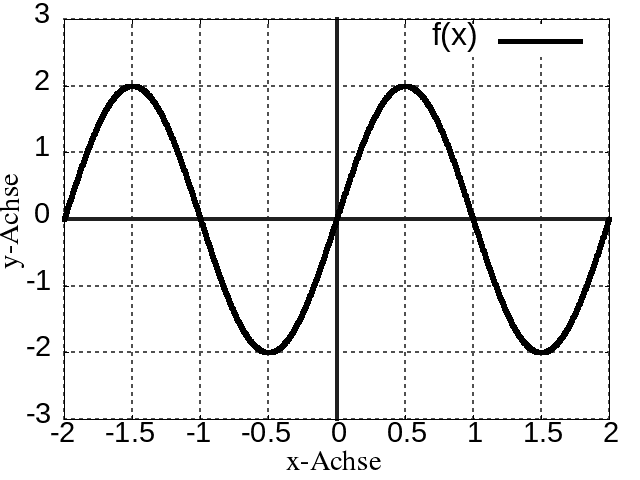
\includegraphics[width=0.35\textwidth]{../tex-snippets/ex-graph-read-1-img-a.png}

\end{multicols}


